\documentclass[frontgrid]{flacards}
\usepackage{color}
\usepackage{tabularx}
\usepackage{graphicx}
\usepackage{amsmath}
\usepackage{pdfpages}

\definecolor{light-gray}{gray}{0.75}

\newcommand{\frontcard}[1]{\textcolor{light-gray}{\colorbox{light-gray}{$#1$}}}
\newcommand{\backcard}[1]{#1} 

\newcommand{\flashcard}[1]{% create new command for cards with blanks
    \card{% call the original \card command with twice the same argument (#1)
        \let\blank\frontcard% but let \blank behave like \frontcard the first time
        #1
    }{%
        \let\blank\backcard% and like \backcard the second time
        #1
    }%
}

\begin{document}

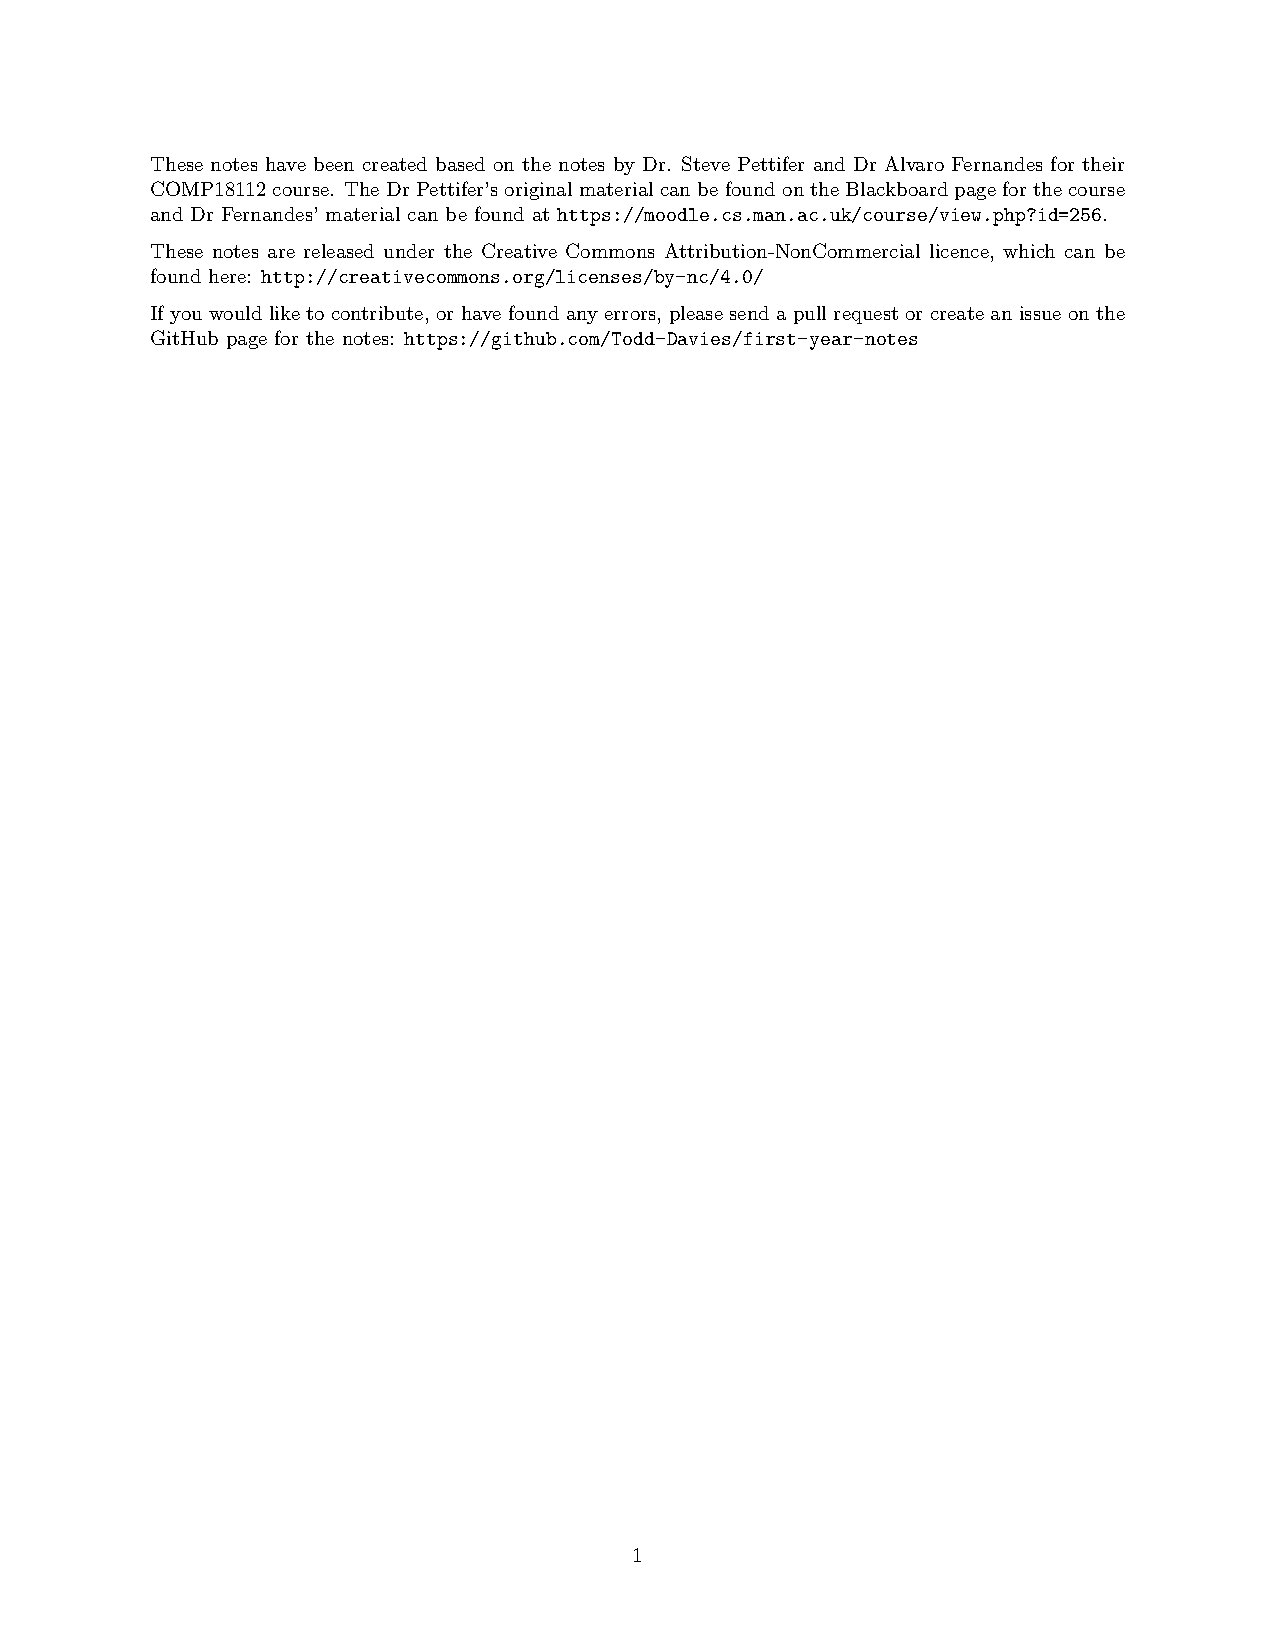
\includepdf[pages={1}]{attribution.pdf}

\newpage

\pagesetup{2}{4} 

%===============================================================================
% Lecture II - Axioms and fallacies of distributed computing
%===============================================================================

\card{
	Define bandwidth.
}{
	Bandwidth measures the maximum amount of data that can be communicated
	within a certain amount of time.
}

\card{
	Define throughput.
}{
	Throughput measures the actual rate at which messages are communicated.
}

%===============================================================================
% Lecture III/IV - Transparency
%===============================================================================

\card{
	On a graph diagram of a distributed system, what is represented by the nodes
	on the graph?
}{
	The physical nodes of the network (individual systems). Each can host
	multiple processes and resources.
}

\card{
	Name some properties of edges that connect the nodes in a graph of a
	distributed system.
}{
	The type of connection (wired/wifi/mobile data etc).\\

	The bandwidth.

	The latency.
}

\card{
	Why is it that even though connections between nodes can be implemented in
	different ways (such as wifi or Ethernet), they can be treated as the same?
}{
	The implementation details of each connection is abstracted away by many
	layers of protocols.
}

\card{
	Name the eight axioms of distributed systems.
}{
	\begin{tabularx}{0.5\textwidth}{lX}
		$\cdot$ & Latency is greater than zero.\\
		$\cdot$ & Bandwidth is less than infinite.\\
		$\cdot$ & Transport cost is greater than zero.\\
		$\cdot$ & There is more than one administrator.\\
		$\cdot$ & The network topology can and will change.\\
		$\cdot$ & The network is not homogeneous (the nodes and edges differ).\\
		$\cdot$ & The network is not secure.\\
		$\cdot$ & The network is not reliable.\\
	\end{tabularx}
}

\card{
	Why is transparency desirable in a distributed system?
}{
	It allows us to design systems as though the distributed axioms were false.
}

\card{
	What is transparency of location? How can we achieve it?
}{
	An attempt to hide the need to know of where a specific resource is
	physically located.\\
	Use DNS servers to map host names to IP addresses.
}

\card{
	What is transparency of migration? How can we achieve it?
}{
	When a host moves location in the network, we shouldn't need to know the
	details	of the move.\\
	The DNS architecture implements this, though if a resource keeps moving,
	then the route through the network and therefore the latency of the
	connection to the host is hard to predict.
}

\card{
	What is transparency of relocation? How is it achieved?
}{
	Transparency of relocation is when parts of the system move while they are
	being accessed. This is hard to mitigate, and is often a problem with mobile
	phone communications.
}

\card{
	What is transparency of replication. How is it achieved?
}{
	When there is more than one physical resource that does the same job, which
	one do we use? It is hard to achieve.
}

\card{
	What is transparency of access? How is it achieved?
}{
	Transparency of access is the ability to not care about how a node is
	implemented. This is often achieved using protocols and API's and
	middleware.
}

\card{
	What is transparency of concurrency?
}{
	Different users shouldn't need to know that others are using the same
	resource and may be competing for its time. Atomic operations and enforcing
	consistency are ways to achieve this, but this can force users to wait on
	each other (deadlock, livelock etc).
}

\card{
	What is deadlock?
}{
	When two different processes are unable to progress since each is waiting
	for information from the other.
}

\card{
	What is livelock?
}{
	When two processes change with respect to one another so that neither can
	make progress.
}

\card{
	What is transparency of failure? How is it achieved?
}{
	Users should not know that a specific node has failed or has recently had
	downtime. Hard to ensure, since sometimes slow connections are
	indistinguishable from failed nodes.
}

%===========================================================================
% Lecture VIII - Systems Software Evolution
%===========================================================================

\card{
	Define systems software.
}{
	The underlying level of software which allows applications to perform their
	tasks efficiently. Examples include device drivers and the operating system.
}

\card{
	Describe the start of the mainframe era.
}{
	\begin{tabularx}{0.5\textwidth}{lX}
		- & Hardware was vastly more expensive than people.\\
		- & Only single user programs.\\
		- & Programs had to be written every time they were to be run.\\
	\end{tabularx}
}

\card{
	What advances were made during the mainframe era?
}{
	\begin{tabularx}{0.5\textwidth}{lX}
		- & The ability to store programs was developed.\\
		- & Batch processing, where jobs would be written to a queue to be
			executed. Lost the ability to debug.\\
		- & Use interrupt handlers and buffers to allow the CPU and IO to work
			in parallel.\\
		- & Multiprogramming so that one program has the CPU and another has the
			IO to enable full resource utilisation.
	\end{tabularx}
}

\card{
	What is the danger of multiprogramming?
}{
	One program could potentially have access to data in other programs, which
	could present security/compatibility concerns. Memory protection is used so
	that programs can only read and write stuff they own.
}

\card{
	What three things can help multiprogramming be effective?
}{
	\begin{tabularx}{0.5\textwidth}{lX}
		- & Fairness policies that impose limits on how much resources jobs 
			should use\\
		- & Schedulers that aim to minimise the time it takes to complete jobs,
			by reducing their response and turnaround time.\\
		- & Preemptive scheduling will temporarily stop jobs if they are hogging
			resources.\\
	\end{tabularx}
}

\card{
	How does the scheduler make decisions about programs?
}{
	Give them priority levels.
}

%===============================================================================
% Lecture IX - Systems Software Evolution: From PCs to Smartphones
%===============================================================================

\card{
	In the beginning of the PC era, what was a typical PC like?
}{
	Everything was cut back with just a single user in mind; no timesharing,
	multiprogramming or protection in the OS, few resources such as memory and
	CPU power etc.
}

\card{
	What happens to the price of PC's during the PC era?
}{
	Price falls due to commoditization and competition.
}

\card{
	How does the usage of PC's change during the PC era?
}{
	They become used for more simple tasks such as word processing, rather than
	number crunching and enterprise processing.
}

\card{
	What does WIMP stand for and when was it introduced?
}{
	Windows, Icons, Menus, Pointer\\ \vspace{1em}
	The WIMP system became common during the PC era.
}

\card{
	What drove an increase in security focus during the PC era?
}{
	The fact that sharing data over networks was becoming increasingly common,
	which exposed security risks. Authentication and authorisation methods were
	therefore developed.
}

\card{
	What are the four standard layers of the network protocol stack?
}{
	\begin{tabularx}{0.5\textwidth}{lX}
		{\bf Name} & {\bf Example}\\
		Application Layer & {\tt HTTP}, {\tt POP}, {\tt SSL}\\
		Transport Layer & {\tt TCP}, {\tt UDP}\\
		Internet Layer & {\tt IP}, {\tt ICMP}, {\tt IGMP}\\
		Link Layer & {\tt ARP}, {\tt Ethernet}, {\tt DSL}, {\tt ISDN}\\
	\end{tabularx}
}

\card{
	When did middleware start to become widely used?
}{
	At the beginning of the web era. API's are used to provide a generic
	interface between the OS and programming languages so that system calls are
	no longer needed. The OS must support middleware rather than implementing
	functions itself.
}

\card{
	In the device era, CPU cycles, storage space and power is all limited. How
	is this overcome?
}{
	Make use of connectivity to servers to offload computation somewhere else.
	This is called the cloud.
}

\card{
	Since there are millions of requests sent to data centres in the device era,
	how is the demand handled?
}{
	Elastically scalable architectures made up of commodity hardware are developed
	along with middleware such as hadoop and map reduce in order to allow for
	massively parallel computation.
}

%===============================================================================
% Lecture X - Distributed Systems: Contrasted with Centralized Ones
%===============================================================================

\card{
	What is the aim of the operating system with regard to resource management?
}{
	To make the most efficient use of the available resources as possible.
}

\card{
	How is memory access controlled by the operating system?
}{
	\begin{tabularx}{0.5\textwidth}{l X}
		- & The OS assigns a {\bf unique identity} to each process.\\
		- & Each process is then assigned an {\bf address space}\\
		- & The OS ensures each process $P$ has a single address space $A$ that
		    is exclusive to that process.
	\end{tabularx}
}

\card{
	Why is it important that a process only have access to isolated areas of
	memory?
}{
	So that processes cannot interfere with each others memory, because of a
	bug or malicious intent.
}

\card{
	Each process executes in a sequential manner, what is a disadvantage of
	this?
}{
	If there was some task that took ages to do, say an API request over a slow
	network connection, then it might be sensible to execute other tasks (maybe
	preparing data for another API request) while the current task is executing
	(i.e. make the tasks concurrent). Due to the sequential nature of processes,
	this is not done.
}

\card{
	What is a {\bf scheduling policy} with regard to operating systems?
}{
	A method of granting each process a time during which it is executed,
	enabling multiple processes to execute in a concurrent fashion, even though
	there may be only one physical set of resources.
}

\card{
	Describe forking.
}{
	When a process forks (through an OS system call) the following happens:
	\begin{tabularx}{0.5\textwidth}{l X}
		- & A child process is created\\
		- & It is given a copy of the parent process's address space, though
		    each address space is distinct.\\
		- & This causes two copies of the process to be active concurrently.
	\end{tabularx}
}

\card{
	Describe threading.
}{
	When a new thread is created in a process:
	\begin{tabularx}{0.5\textwidth}{l X}
		- & A new child process is created\\
		- & The address space is shared between the child and the parent.\\
		- & The parent and child processes are less isolated, and can therefore
		    interact together easier, however, this can be dangerous and a
		    source of bugs.\\
		- & Since no memory is copied, threading is less expensive than
		    forking.
	\end{tabularx}
}

\card{
	When there are many independent, self-sufficient, autonomous, heterogeneous
	machines working together with spatial separation, what is required to
	facilitate effective working?
}{
	Message exchange over a network, best facilitated with a middleware API to
	abstract away some complexity.
}

%===============================================================================
% Lecture XI - Distributed Systems: Interconnecting them
%===============================================================================

\flashcard{
	A significantly long interconnect (i.e. a \blank{full blown network}) is not
	\blank{cost-neutral}.
}

\card{
	Describe an SISD architecture.
}{
	A single instruction/program, single dataset architecture. An example of
	this is an older, single core PC, where there is only data space (the main
	memory) and there is cost neutral access to it.
}

\card{
	Describe an SIMD architecture.
}{
	A single instruction/program, multiple dataset architecture. This could be
	used to describe a computer with a GPU that is applying {\bf the same}
	transformation to many pixels at once. Access to data is {\bf not} cost
	neutral since the data is being shared amongst different instances of a
	program/instruction.
}

\card{
	Describe a MISD architecture.
}{
	A multiple program/instruction, single dataset architecture. Though not as
	useful as other architectures, a sample MISD use case is in safety critical
	systems where two independent processors could compute the same function on
	the same data and check their results against each other.
}

\card{
	Describe a MIMD architecture.
}{
	A multiple instruction/program, multiple dataset architecture. Here, a
	form of interconnect will bind together several self sufficient autonomous
	components. The interconnect isn't cost neutral, but the gain in
	functionality is great. This architecture is widely used in applications
	such as clouds, clusters, and even multi-core PC's.
}

\card{
	Describe the advantages of a MIMD architecture.
}{
	A MIMD architecture allows you to scale out instead of up. An architecture
	that lets you scale out is one where you can add more hardware (such as
	servers/hard drives) as opposed to upgrading existing hardware which is
	scaling up (i.e. increasing the RAM in a server).
}

\card{
	What architecture is this:\\
	\includegraphics[scale=0.3]{images/SISD}
}{
	SISD
}

\card{
	What architecture is this:\\
	\includegraphics[scale=0.3]{images/SIMD}
}{
	SIMD
}

\card{
	What architecture is this:\\
	\includegraphics[scale=0.3]{images/MISD}
}{
	MISD
}

\card{
	What architecture is this:\\
	\includegraphics[scale=0.3]{images/MIMD}
}{
	MIMD
}

\flashcard{
	MIMD architectures (aka \blank{shared-nothing} architectures) often
	communicate over a \blank{network} such as \blank{the Internet} that exists
	\blank{separately} to the architecture itself.
}

\card{
	What does vBNS stand for?
}{
	Very high performance Backbone Network Service.
}

\card{
	What does OC stand for? What does OC-n mean?
}{
	OC stands for Optical Carrier.\\\vspace{1em}
	OC-n = $n \times 54.84 \textrm{Mbit/s}$
}

\card{
	What is the network protocol stack?
}{
	Layers of protocols that talk to each other to facilitate network
	connectivity.
}

\card{
	What are the five layers of the protocol stack?
}{
	\[
		\begin{split}
			\textrm{Application} &\leftrightarrow \textrm{Transport}\\
								 &\leftrightarrow \textrm{Internet}\\
								 &\leftrightarrow \textrm{Link}\\
								 &\leftrightarrow \textrm{Physical}
		\end{split}
	\]
}

\card{
	Describe the job of the application layer.
}{
	To take care of specific application needs such as sending emails or HTTP
	requests.
}

\card{
	Describe the job of the transport layer.
}{
	To make sure that there is a logical channel for messages to flow through.
	E.g. TCP
}

\card{
	Describe the job of the Internet layer.
}{
	To make sure packets sent over the network reach their intended destination.
	E.g. IP
}

\card{
	What is the job of the link layer?
}{
	Making sure that there is a physical channel to pass data through. E.g. MAC
}

\card{
	What is the job of the physical layer?
}{
	To physically pass messages between networked components. Deals with all
	the physics etc. E.g. Wifi
}

\card{
	What is the hourglass model?
}{
	Very varied application layers at the top of the network stack (emails,
	streaming video etc), as simple protocols as possible in the middle of the
	stack, and very varied physical devices at the bottom (bluetooth, wifi,
	optical fibre etc).
}

\card{
	What is a packet switched network?
}{
	\begin{tabularx}{0.5\textwidth}{l X}
		- & A network of networks formed by interconnecting routers.\\
		- & The message is divided into packets before transmission.\\
		- & The packets are reconstituted into the original message at
			reception.\\
		- & Packets may take varied routes while in transit, and be grouped with
			unrelated packages from other messages.\\ 
	\end{tabularx}
}

\card{
	What is the job of a router in a packet switched network?
}{
	To examine the header data in each packet and send the packet on to another
	router in the network that is closer to the packet's destination, while
	accounting for how saturated datapaths are in order to find an efficient
	route.
}

\card{
	What are some differences between TCP and UDP?
}{
	\begin{tabularx}{0.5\textwidth}{l X}
		- & TCP is connection oriented, UDP isn't.\\
		- & TCP is reliable and ensures that messages arrive at their
				destination, intact and in the right order. If the messages do
				not arrive, then it will be known. UDP only provides a
				corruption guarantee.\\
		- & UDP is more lightweight than TCP and is better for quick
			communication where the occasional loss or out of order packet isn't
			a problem.
	\end{tabularx}
}

\card{
	What is packet encapsulation?
}{
	Each layer of the networking stack wraps messages in a packet that contains
	information about the packet. By the time the packet has descended to the
	physical layer, then it may have many layers of headers and metadata.
}

\card{
	Why does packet encapsulation enable flexibility?
}{
	It doesn't matter about what information the packet is carrying, at each
	layer of the network stack, the callee layer has multiple choices of what
	protocol to use for the next level on the stack, and simply chooses the most
	convenient/suitable one.
}


%===============================================================================
% Lecture XII - Distributed systems - Architectural Paradigms
%===============================================================================

\card{
	What does IPC stand for?
}{
	Inter-Process Communication
}

\flashcard{
	A successful communication between processes must consist of one process
	being \blank{ready to send} coinciding with another process being
	\blank{ready to receive}. This is non trivial with \blank{independent
	timelines}.
}

\card{
	Describe Direct Message Exchange as a Distributed Architecture.
}{
	In order to communicate, the sending process must be in a position to send
	and the receiving process must be in a position to receive messages. Upon
	receiving a message, a process may interpret it and then respond.
}

\card{
	What is asymmetric DME?
}{
	Direct Message Exchange	where processes are assigned special roles such as a
	client or server in order to simplify the process. All the server has to do
	is wait for messages and all the client has to do is send messages.
}

\card{
	What is a symmetric DME?
}{
	Direct Message Exchange	where no special roles are assigned to processes,
	also known as a peer-to-peer architecture. Event synchronisation is less 
	simple with a symmetric DME than with an asymmetric one.
}

\card{
	What is a MME architecture?
}{
	A Mediated Message Exchange architecture is one where inter process
	communication goes through a central middleware component (often referred
	to as message orientated middleware). Allows for event synchronisation to be
	decoupled in time since the middleware is always avalible.
}

\flashcard{
	If a message in a MME architecture goes to more than one destination it is
	described as being a \blank{public subscribe system}, if messages only go
	to one destination, then the system is described as being \blank{point to
	point}.
}

\card{
	What is RPC?
}{
	A remote procedure call is similar to a message, though the data is passed
	as parameters to a method. It is often facilitated by middleware such as
	{\tt CORBA}. When OOP principles are involved, RPC is called {\bf Remote
	Method Invocation (RMI)}.
}

\card{
	Why is middleware such as MME, RPC and RMI beneficial?
}{
	They raise the level of abstraction at which we can build and engineer
	distributed systems.
}

%===============================================================================
% Lecture XIII - Distributed Systems: Synchronization and Blocking Primitives
%===============================================================================

% This lecture is crap

%===============================================================================
% Lecture XIV - Distributed Systems: Socket-Level Client-Server Systems
%===============================================================================

\card{
	What is a protocol?
}{
	A set of rules for inter process communication that stipulates the precise
	sequence of events that must be enacted by the communicating processes for
	them to successfully communicate.
}

\flashcard{
	The operating system provides an \blank{API (application programming
	interface)} for IPC.
}

\card{
	Name two important OS services relied on by an API for IPC in the OS.
}{
	\begin{tabularx}{0.5\textwidth}{lX}
		- & Keeping network buffers.\\
		- & Providing synchronisation mechanisms.
	\end{tabularx}
}

\flashcard{
	Sockets are \blank{an additional layer on} the network stack provided by 
	the operating system to abstract away the details of \blank{low level IPC}.
	In this manner, communicating processes \blank{read and write} to each
	others sockets in an \blank{I/O} style manner.
}

\card{
	What the lifecycle of a client side socket?
}{
	\begin{tabularx}{0.5\textwidth}{lX}
		1. & The socket is created for a given transport protocol (E.g. TCP) and
		     Internet protocol (E.g. IPv6)\\
		2. & A connection is then opened with the desired IP/port combination.\\
		3. & The client then sends a request through the socket and waits for a
		     response (through the same socket).\\
		4. & The server then replies with a response, which may come in
		     chunks.\\
		5. & Once the response has been received, the socket is closed and
		     discarded.
	\end{tabularx}
}

\card{
	How is a server side socket {\bf set up}?
}{
	\begin{tabularx}{0.5\textwidth}{lX}
		1. & The socket is created for a given transport protocol (E.g. UDP) and
		     Internet protocol (E.g. IPv4)\\
		2. & Set the options for the socket, such as whether it is reusable.\\
		3. & Bind the socket to the address and port to listen on.\\
		4. & Start listening for connections, set the maximum number of
		     connections to leave in a queue if there is a significant load.\\
	\end{tabularx}
}

\card{
	How are connections handled in a server side socket?
}{
	\begin{tabularx}{0.5\textwidth}{lX}
		1. & The socket waits to accept a connection.\\
		2. & When a connection is accepted, a new socket is created with the IP
		     address and port of the connecting client in it.\\
		3. & The server process then handles the new connection as appropriate,
		     e.g. by spawning a thread and passing the socket to that thread.\\
		4. & The server process can then continue in its loop (back to stage
		     1).\\
	\end{tabularx}\\
	\vspace{1em}
	Note that spawned sockets and their handlers need to be closed
	properly after the client has disconnected.
}

%===============================================================================
% Lecture XXII - Massive Distribution for Performance
%===============================================================================

\card{
	When is the benefit most useful from massively parallelising a task?
}{
	When the data can be partitioned and multiple computers can work on the data
	independently then the performance benefits are most significant.
}

\card{
	When a task is divided into parts for execution on many machines, what
	challenges are presented in doing this?
}{
	\begin{tabularx}{0.5\textwidth}{lX}
		- & What if we have more workers than tasks, or more tasks than
		    workers?\\
		- & How do we know if all the workers have finished?\\
		- & How do we aggregate the results of the workers?
	\end{tabularx}
}

\flashcard{
	Operations that seem \blank{atomic} may actually \blank{compile down into
	several different steps} further down the software stack. This can cause
	problems if seemingly atomic operations are running concurrently, since they
	could \blank{interleave} further down the stack and interfere with each
	other.
}

\card{
	What is a synchronisation primitive?
}{
	A language construct that provides access to a shared variable with a
	OS/hardware guaranteed atomicity. Used to enforce execution sequences.
}

\card{
	What is a barrier?
}{
	A synchronisation primitive that forces multiple processes to wait at the
	barrier until they have all reached the barrier. For this to be efficient,
	all the processes must reach the barrier more or less at the same time.
}

\card{
	When can an expression be split into multiple parts?
}{
	When independent branches of the expression do not have any shared state,
	they can be executed in any order or parallelized.
}

\card{
	We can split the following expression into {\tt x + y} and {\tt a + b} to be
	parallelized. What is the blocking point?\\
	\vspace{1em}
	{\tt c = (a+b) * (x+y)}
}{
	The assignment to {\tt c}.
}

\flashcard{
	When designing tasks for parallelized computation, the goal is to identify
	and eliminate as many \blank{synchronisation points} as possible and
	eliminate them, so that the \blank{independent tasks} can be carried out on
	different machines as \blank{efficiently} as possible.
}

\card{
	How does map reduce make it easier to make tasks independent?
}{
	By limiting the expressiveness of the computation of the tasks so they can be
	more easily parallelized.
}

\card{
	Why are functional programs easy to parallelize?
}{
	Since pure functions are side effect free, meaning that two functions used
	in the same expression are guaranteed not to share state and so can be
	parallelized safely.
}

\flashcard{
	The {\tt map} function takes \blank{a collection {\tt [i\_1, ..., i\_n]}}
	and \blank{a function {\tt f}} and returns \blank{the collection
	{\tt [f(i\_1), ..., f(i\_n)]}}
}

\card{
	Why is {\tt map} parallelizable?
}{
	Since the function applying to the collection can be applied to each item in
	the collection independently, and is side effect free.
}

\flashcard{
	{\tt Reduce} takes a \blank{binary associative function {\tt f(x,y)}} and
	\blank{a collection {\tt [i\_1, ..., i\_n]}}, and returns\\
	\blank{f(i\_n,f(...,f(i\_0, i\_1))...)}
}

\card{
	How can {\tt reduce} be parallelized?
}{
	Have different parts of the list run in different tasks and then apply the
	function to the result of tasks to combine them together again at the end.
}

\card{
	How is the map and the reduce stage synchronised with each other in Hadoop
	and other map-reduce engines?
}{
	With a barrier.
}

\card{
	What useful features do map-reduce engines such as Hadoop implement?
}{
	\begin{tabularx}{0.5\textwidth}{lX}
		- & Load balancing\\
		- & Fault tolerance\\
		- & Splitting, spawning and merging of tasks
	\end{tabularx}
}

\card{
	Just look over this one. Make sure you understand how the map-reduce
	architecture works.
}{
	\includegraphics[scale=0.25]{images/map-reduce}
}

%===============================================================================
% Lecture XXIII - Services over the Web 
%===============================================================================

\flashcard{
	If you have a network built of identical worker nodes, each working on a
	partition of some dataset, then the computation is \blank{not inherently
	distributed}, and could be referred to as a form of \blank{divide-and-
	conquer} strategy. However, if you have a network built of heterogeneous
	workers that are operating on data that are not partitions of a single
	dataset, then you have \blank{an inherently distributed} computation, which
	is a case of \blank{unite-and-conquer}.
}

\flashcard{
	A distributed system working within one company is referred to as an
	\blank{enterprise application integration} (EAI) system.
}

\flashcard{
	A distributed system spanning multiple companies is referred to as an
	\blank{business to business integration} (B2B) system.
}

\card{
	What is an RIA?
}{
	A Rich Internet Application (e.g. Gmail)
}

\card{
	What is a web mashup?
}{
	A lightweight web application that combines processing and data resources
	from different sources into a single application.
}

\flashcard{
	The {\tt WS-*} view is a family of standards that all start with
	`{\tt WS-}'. It is an example of a \blank{Service Oriented Architecture}
	(SOA), and interactions are defined by a \blank{higher up} protocol called
	\blank{SOAP}. {\tt WS-*} interactions sit on top of other protocols such as
	{\tt HTTP} or {\tt SMTP}.
}

\card{
	What does REST stand for?
}{
	REpresentational State Transfer.
}

\card{
	How does REST operate?
}{
	The sender places a payload into a request such as {\tt HTTP Post}, which is
	then sent to a receiver. The receiver will then respond via the same method
	with the response (if any).
}

\flashcard{
	In a RESTful service, interactions between components are \blank{operations
	on resources}, and the service is seen as a \blank{Resource Oriented
	Architecture} (\blank{ROA}).
}

\card{
	What (according to the lecture slides) features do SOAP API's offer to
	justify them being more heavyweight?
}{
	\begin{tabularx}{0.5\textwidth}{lX}
		- & Security, authentication and authorisation\\
		- & Robust addressing and reliable messaging\\
		- & Transactional semantics (fault tolerance features)\\
	\end{tabularx}
	\\
	\vspace{1em}
	The above are very useful in EAI and B2B contexts.
}

\card{
	This is the {\it real difference} between REST and SOAP API's.
}{
	\includegraphics[scale=0.3]{images/rest-vs-soap}
}

%===============================================================================
% Lecture XXIV - The Web as a Massive Distributed Database
%===============================================================================

\flashcard{
	In the Web of Data view, the web is \blank{a massive distributed database}.
}

\card{
	Why is the data exposed by API's often hard to use with processing
	algorithms?
}{
	Even though the data might be able to be parsed (i.e. if it's in JSON), the
	semantics of the data are still unclear since different API's follow
	different specifications and therefore it is hard to extract useful,
	unambiguous data.
}

\flashcard{
	The Web of Data (WoD) is a \blank{graph}, similar to a relational database,
	but with no predefined \blank{schema}. The \blank{edges} between
	\blank{nodes} define relationships in the data.
}

\card{
	What does RDF stand for? What is it?
}{
	Resource Description Language. There are various implementations of RDF,
	such as XML, turtle format, N-triples format etc.
}

\flashcard{
	In the WoD, we have \blank{linked} data where resources are URI-assigned
	nodes, linked by \blank{explicitly declared relationships}.
}

\card{
	What does OWL mean?
}{
	Web Ontology Language
}

\card{
	Describe the {\bf follow your nose} approach to querying the web of data.
}{
	\begin{tabularx}{0.5\textwidth}{lX}
		- & Select and connect to an initial seed URI.\\
		- & Send it your declarative query.\\
		- & Iterate through the triples in the result and decide whether to 
		    hyperlink the triple.\\
		- & Now you can do more queries if needed to expand your results set.
	\end{tabularx}
}

\card{
	What is data source federation?
}{
	Middleware that emulates one virtual database from many physical (local)
	data sources. It does this by constructing many smaller queries on its
	local data sets based on a global query that it has been given and then 
	compiling the results together as a response. This removes the need for
	decision making such as in the follow your nose approach to traversing the
	WoD.
}


%===============================================================================
% Steve's stuff
%===============================================================================

\flashcard{
	MAC addresses are made up of a \blank{24 bit OUI} number purchased by 
	manufacturers from the \blank{IEEE}, and another \blank{24 bit NIC} number
	issued by \blank{the manufacturer}. In this way, the \blank{manufacturer}
	needs to ensure only that the second number	needs to be unique.
}

\card{
	MAC address stands for? Why is it silly to call a MAC address an `address'?
}{
	Media Access Control\\
	\vspace{1em}
	An address contains information about the whereabouts of an entity. A MAC
	address is really just a Unique Identifier.
}

\flashcard{
	An IP (\blank{Internet Protocol}) address serves two purposes; as a
	\blank{unique identifier} and as an indication of \blank{where a device is
	on a network}. The \blank{IANA} (\blank{Internet Assigned Numbers
	Authority}) assigns blocks of addresses to regional authorities, meaning
	that IP addresses do have some \blank{geographical} relationship.
}

\card{
	What does DNS stand for?
}{
	Domain Name Server.
}

\flashcard{
	When a DNS server is given a \blank{domain name} to translate into an
	\blank{IP} address, it looks to see if it already has the answer in its
	cache and returns it if so. Otherwise, it will \blank{propagate the request
	up} the hierarchy until it does find an answer.
}

\card{
	How does the DNS system control how caching is used?
}{
	Each DNS record has a TTL (Time To Live), which dictates how long the server
	should retain the record in its cache before replacing it from higher up the
	hierarchy. TTL values can be from seconds up to 68 years, or never.
}

\card{
	What does {\tt HTTP} stand for?
}{
	HyperText Transfer Protocol
}

\flashcard{
	The web is a \blank{stateless} protocol in order to save the resources that 
	would be required if a \blank{connection} was to be left open for the
	duration of a session.
}

\card{
	If {\tt HTTP} is a stateless protocol, then how is state retained on the
	web?
}{
	The web server retains the state, not the {\tt HTTP} protocol.
}

\card{
	What is the function of the {\tt HEAD} HTTP verb?
}{
	Provides metadata about a resource. Just like a {\tt GET} request, except
	the body of the request is not returned. Used to let clients know if cached
	data has changed.
}

\card{
	What is the function of the {\tt GET} HTTP verb?
}{
	Gets a resource from the server.	
}

\card{
	What is the function of the {\tt POST} HTTP verb?
}{
	Submits data to the server. The state of the server may change as a result
	of a {\tt POST} request.
}

\card{
	What is the function of the {\tt OPTIONS} HTTP verb?
}{
	Returns the list of commands supported by the server.
}

\card{
	What does the 'store and forward' model mean?
}{
	When a message needs to be transmitted along a network, but not all the
	nodes along the path may be active at the same time. Consequently, the
	message is stored by each node until it has been confirmed to have been
	received by the next node.
}

\card{
	What is the SMTP protocol?
}{
	The Simple Mail Transfer Protocol is a method for sending email. It is a
	text-based, stateful, connection based protocol, so a connection to the
	server must be opened before the message can be transferred, and then
	closed again after.
}

\card{
	What is the POP protocol?
}{
	The Post Office Protocol. Lets you read and delete emails from a server. If 
	a message is not deleted, then it will stay unread for the next time (though
	a client may choose just not to download it next time). Like SMTP, POP is
	text based, stateful and connection based.
}

\card{
	What is IMAP?
}{
	The Internet Message Access Protocol is an email protocol that lets you see
	the head of a message rather than just having to download the whole thing.
	This means you can more easily cache emails on a client and then download
	any changes that have occurred. It also lets users have multiple inboxes,
	server side searching and it deals with attachments better than POP.
}

\card{
	What are the four Coffman conditions?
}{
	\begin{tabularx}{0.5\textwidth}{>{\bfseries}l X}
		Mutual Exclusion & There must be at least one resource that cannot be
						   shared.\\
		Hold and Wait &    A process is currently holding one (or more)
						   resource(s), and is waiting for another resource 
						   currently held by another process.\\
		No preemption &    Nothing can force a process to give up a resource
						   unless it does so willingly.\\
		Circular wait &    There must be a cycle of dependencies so that
		                   processes are waiting for each other to relinquish
		                   resource control before they themselves do.
	\end{tabularx}
}

\card{
	What is deadlock?
}{
	A deadlock is a situation in which two or more competing actions are each
	waiting for the other to finish, and thus neither ever does.
}

\card{
	What is livelock?
}{
	Livelock is similar to deadlock except that the states of the system 
	constantly change with regard to each other, but they never actually
	progress.
}

\card{
	What is resource starvation?
}{
	 Starvation is where a process is perpetually denied necessary resources.
	 Without those resources, the program can never finish its task.
}

\card{
	What is the difference between thin and thick clients?
}{
	A thin (or dumb) client will do little processing, and merely just echo or
	display whatever the server tells it to. A thick client on the other hand 
	will have functionality built into it that is able to work independently of
	the server.
}

\card{
	Describe `reduction to absurdity'.
}{
	This is a type of argument where an idea is shown to be false by showing
	that an absurd result can be obtained by the acceptance of the idea.
}

\card{
	Give an example of `reduction to absurdity'.
}{
	\begin{tabularx}{0.5\textwidth}{lX}
		- & Assume that a successful coordinated action occurs as a result of
		    messages being passed with communicating parties.\\
		- & Assume the last message in the sequence is lost.\\
		- & If the action still succeeds, then the last message was
		    unimportant.\\
		- & Repeat until no messages are exchanged.\\
		- & Our initial assumption was clearly wrong!
	\end{tabularx}
}

\card{
	With a Lamport clock, how is the clock of $A$ affected if $B$ sends $A$ a
	message?
}{
	\begin{tabular}{l}
		{\tt if LCy < (LCx + 1):}\\
		\hspace{2em}{\tt LCy = LCx + 1}
	\end{tabular}
}

\card{
	Describe the purpose of a mutex.
}{
	A mutex ensures that two processes do not enter into a critical section of
	their execution at the same time and therefore prevents race conditions and
	enables the safe sharing of resources.
}

\card{
	What is a critical section?
}{
	A critical section is a sequence of actions that should execute in an atomic
	matter. That is to say that if the critical section does not succeed, then
	the state of the system should be exactly the same as when the critical
	section started.
}

\card{
	Describe the two-phase commit.
}{
	\begin{tabularx}{0.5\textwidth}{lX}
		1 & A coordinator node wishes all of the nodes to perform an action.\\
		2 & It sends a request to all of the other nodes.\\
		3 & The other nodes attempt to perform the action, and reply with
			{\tt commit} or {\tt abort} depending on whether they to performed
			the action.\\
		4a& If any one of the nodes replied {\tt abort}, then the coordinator
			node will reply {\tt global\_abort} and all the nodes will roll back
			their state to that of the start of the transaction.\\
		4b& If all the nodes replied {\tt commit}, then the coordinator node
			will send {\tt global\_commit} and the nodes will retain their
			current	state.\\
	\end{tabularx}
}

\card{
	Describe the bully algorithm.
}{
	\begin{tabularx}{0.5\textwidth}{lX}
		1 & A node wants to be a coordinator, so it sends a message to all the
			other nodes with its number.\\
		2 & All the other nodes will only reply if they have a higher number. If
			they do, they will start another election.\\
		3 & The process continues until a node receives no replies, and is
			therefore the coordinator, at which point, it will inform all the
			other nodes of this.\\
	\end{tabularx}
}

\card{
	Describe Cristian's algorithm?
}{
	In order to synchronise the clocks of two systems, one system $S$ will send
	its time to another system $C$. After receiving the request from $S$, $C$
	will then reply with its own clock time. When $S$ receives this, then it
	will set its clock to be the time that $C$ sent added to the round trip time
	(discernible from $C$'s reply) divided by two.
}

\card{
	Describe the Berkly algorithm.
}{
	\begin{tabularx}{0.5\textwidth}{lX}
		1 & A master node is chosen.\\
		2 & The master polls the other nodes for the time.\\
		3 & The master observes the round trip time for each state, and
			estimates the time of each client.\\
		4 & The master then averages out the clock times and sends each node a
			message containing the difference that it is from the average.
	\end{tabularx}
}

\card{
	What is an overlay network?
}{
	A virtual network that is superimposed onto an existing network. Nodes in
	an overlay network can be thought of as connected by virtual links that may
	be composed of many actual physical links in the real network.
}

\card{
	How was Napster's distributed architecture organised?
}{
	Napster had a central server which acted as a file directory/search engine
	that enabled peers to connect to each other and exchange files.
}

\card{
	How was Gnutella's network organised?
}{
	\begin{tabularx}{0.5\textwidth}{lX}
		- & To join, you have to have the IP address of a node in the network.\\
		- & Queries for files are `flooded' around the network, with peers
		    asking their neighbours if they don't have the file.\\
		- & This was inefficient, since if the peers didn't have the file, then
		    the request would go around the whole network before failing.\\
	\end{tabularx}
}


\card{
	How was KaZaa's network organised?
}{
	\begin{tabularx}{0.5\textwidth}{lX}
		- & There were two types of nodes; normal and supernodes.\\
		- & Nodes would be promoted to supernodes if they had sufficient uptime
		    and bandwidth (though they could demote themselves if they didn't
		    want to be a supernode).\\
		- & Supernodes would take on higher level tasks for the child nodes,
		    such as indexing files and sharing data with other supernodes.\\
		- & Supernodes improved querying substantially, since failed queries
		    needed only to go around the supernodes, not all of the nodes.\\
	\end{tabularx}
}

\card{
	Why has BitTorrent been immune to successful prosecution?
}{
	The BitTorrent protocol doesn't know about the contents of files, only their
	hash code. This means you can't search for torrents based only on the files
	themselves (though you can use a third party indexing service such as 
	pirate bay). Also, the protocol is completely distributed, so BitTorrent
	can be argued to be just an efficient file sharing mechanism rather than a
	copyrighting infringing mechanism.
}

\card{
	How does BitTorrent get people to seed content?
}{
	If a client limits its upload speed, then the protocol will throttle the
	download speed to the client accordingly with a `more you give, more you
	get' philosophy.
}

\card{
	How does BitTorrent work?
}{
	\begin{tabularx}{0.5\textwidth}{lX}
		- & Files are split into blocks, by default {\tt 256Kb}.\\
		- & A torrent file is created which contains metadata about the file,
			and a link to a tracker server which will tracks active clients.\\
		- & A client will contact the tracker for a swarm of other clients
			downloading the file, these other clients are called the peer set.\\
		- & If the number of peers in the set drops below 20, then more will be
			requested from the server.
	\end{tabularx}
}

\card{
	Describe BitTorrent's choke/unchoke policy.
}{
	\begin{tabularx}{0.5\textwidth}{lX}
		- & A peer serves the 4 best connected peers in its peer set at any one
		    time.\\
		- & Every ten seconds, the worst of the four is choked if there is a
		    better peer\\
		- & Every thirty seconds, a random peer from the set is unchoked in the
		    hope that it offers good speeds.
	\end{tabularx}
}

\flashcard{
	A hash function maps a \blank{key (the thing you’re searching for)} to a
	\blank{number}, which then allows you to quickly index into a table to find
	the result you want.
}

\card{
	In a ring based hash table, if there are more buckets than nodes, then how
	can we assign all the buckets to at least one node?
}{
	Make nodes responsible for all the buckets below them in the ring until the
	next node.\\
	\includegraphics[scale=0.2]{images/ring}
}

\card{
	In a distributed hash table, how many keys is each node responsible for if
	there are $N$ nodes and $K$ keys?
}{
	$\frac{K}{N}$
}

\flashcard{
	In Chord, a \blank{finger table} is created so that queries don't have to
	go all the way around the ring. The $i^{\textrm{th}}$ entry of a nodes
	finger table contains the address of the successor
	$(n + 2^{i-1} ) mod 2^m$.
}

\card{
	What are the four components of a game engine?
}{
	\begin{tabular}{ll}
		- & Rendering engine\\
		- & Physics engine\\
		- & Networking layer\\
		- & Behaviour module\\
	\end{tabular}
}

\card{
	What were some of the limitations of Doom's gameplay?
}{
	The speed of the gameplay was limited to the speed of the slowest connected
	computer over the network that was being played on. The P2P architecture
	also meant there was no saved state if all the players disconnected.
}

\card{
	How did Quake implement online gameplay?
}{
	There was a server (dedicated or participant) that had the full game state,
	which allowed clients to perform at their own rates, and games to persist if
	clients left. Client side prediction was utilised to reduce network load.
}

\card{
	What is client side prediction?
}{
	Sending information to change the state of a client rather than sending the
	whole new state in order to save bandwidth. E.g. Sending a trajectory
	instead of sending a position ten times per second.
}

\card{
	Why is the Unreal game engine so good?
}{
	It allows developers to `tear off' aspects of the game to be processed
	entirely on the client side, and thus saving bandwidth and server CPU
	cycles. Such aspects may be animations such as explosions or characters
	dying.
}

%===============================================================================
% Misc
%===============================================================================

\card{
	When answering questions, Alvaro wants us to...
}{
	Describe, explain, justify, contrast
}

\end{document} 
